% Template for PLoS
% Version 2.0 July 2014
%
% To compile to pdf, run:
% latex plos.template
% bibtex plos.template
% latex plos.template
% latex plos.template
% dvipdf plos.template
%!TEX encoding = UTF-8 Unicode
% % % % % % % % % % % % % % % % % % % % % %
%
% -- IMPORTANT NOTE
%
% Be advised that this is merely a template 
% designed to facilitate accurate translation of manuscript content 
% into our production files. 
%
% This template contains extensive comments intended 
% to minimize problems and delays during our production 
% process. Please follow the template 
% whenever possible.
% % % % % % % % % % % % % % % % % % % % % % % 
%
% Once your paper is accepted for publication and enters production, 
% PLEASE REMOVE ALL TRACKED CHANGES in this file and leave only
% the final text of your manuscript.
%
% DO NOT ADD EXTRA PACKAGES TO THIS TEMPLATE unless absolutely necessary.
% Packages included in this template are intentionally
% limited and basic in order to reduce the possibility
% of issues during our production process.
%
% % % % % % % % % % % % % % % % % % % % % % %
%
% -- FIGURES AND TABLES
%
% DO NOT INCLUDE GRAPHICS IN YOUR MANUSCRIPT
% - Figures should be uploaded separately from your manuscript file. 
% - Figures generated using LaTeX should be extracted and removed from the PDF before submission. 
% - Figures containing multiple panels/subfigures must be combined into one image file before submission.
% See http://www.plosone.org/static/figureGuidelines for PLOS figure guidelines.
%
% Tables should be cell-based and may not contain:
% - tabs/spacing/line breaks within cells to alter layout
% - vertically-merged cells (no tabular environments within tabular environments, do not use \multirow)
% - colors, shading, or graphic objects
% See http://www.plosone.org/static/figureGuidelines#tables for table guidelines.
%
% For sideways tables, use the {rotating} package and use \begin{sidewaystable} instead of \begin{table} in the appropriate section. PLOS guidelines do not accomodate sideways figures.
%
% % % % % % % % % % % % % % % % % % % % % % % %
%
% -- EQUATIONS, MATH SYMBOLS, SUBSCRIPTS, AND SUPERSCRIPTS
%
% IMPORTANT
% Below are a few tips to help format your equations and other special characters according to our specifications. For more tips to help reduce the possibility of formatting errors during conversion, please see our LaTeX guidelines at http://www.plosone.org/static/latexGuidelines
%
% Please be sure to include all portions of an equation in the math environment, and for any superscripts or subscripts also include the base number/text. For example, use $mathrm{mm}^2$ instead of mm$^2$ (do not use the\textsuperscript command).
%
% DO NOT USE the \rm command to render mathmode characters in roman font, instead use $\mathrm{}$
% For bolding characters in mathmode, please use $\mathbf{}$ 
%
% Please add line breaks to long equations when possible in order to fit our 2-column layout. 
%
% For inline equations, please do not include punctuation within the math environment unless this is part of the equation.
%!TEX encoding = UTF-8 Unicode
% For spaces within the math environment please use the \; or \: commands, even within \text{} (do not use smaller spacing as this does not convert well).
%
%!TEX encoding = UTF-8 Unicode
% % % % % % % % % % % % % % % % % % % % % % % %



\documentclass[10pt]{article}
\usepackage{colortbl}

% amsmath package, useful for mathematical formulas
\usepackage{amsmath}
% amssymb package, useful for mathematical symbols
\usepackage{amssymb}

% cite package, to clean up citations in the main text. Do not remove.
\usepackage{cite}
 
\usepackage{hyperref}

% line numbers
\usepackage{lineno}
 
 % ligatures disabled
\usepackage{microtype}
\usepackage{graphicx} 
 
% \DisableLigatures[f]{encoding = *, family = * }

% rotating package for sideways tables
%\usepackage{rotating}

% If you wish to include algorithms, please use one of the packages below. Also, please see the algorithm section of our LaTeX guidelines (http://www.plosone.org/static/latexGuidelines) for important information about required formatting.
%\usepackage{algorithmic}
%\usepackage{algorithmicx}

% Use doublespacing - comment out for single spacing
%\usepackage{setspace} 
%\doublespacing


% Text layout
\topmargin 0.0cm
\oddsidemargin 0.5cm
\evensidemargin 0.5cm
\textwidth 16cm 
\textheight 21cm

% Bold the 'Figure #' in the caption and separate it with a period
% Captions will be left justified
\usepackage[labelfont=bf,labelsep=period,justification=raggedright]{caption}
 
 % Remove brackets from numbering in List of References
\makeatletter
\renewcommand{\@biblabel}[1]{\quad#1.}
\makeatother


% Leave date blank
\date{}

\pagestyle{myheadings}

%% Include all macros below. Please limit the use of macros.

%% END MACROS SECTION

 
\begin{document}


% Title must be 150 characters or less
\begin{flushleft}
{\Large
\textbf{Evaluating Metagenome Assembly on a Complex Community}
}
% Insert Author names, affiliations and corresponding author email.
\\
 
Sherine Awad $^{1}$, 
Luiz Irber $^{1}$, 
C. Titus Brown $^{1,\ast}$ 

\bf{1} Population Health and Reproduction
University of California, Davis, Davis, CA, USA 
 
 
$\ast$ E-mail:  ctbrown@ucdavis.edu 
\end{flushleft}

% Please keep the abstract between 250 and 300 words
% Please keep the abstract between 250 and 300 words
\section*{Abstract}
NEEDS ENHANCEMENTS

Motivation: With the emergence of de novo assembly, several work have been to done to assemble metagenomic data from de novo. Several assemblers exist that are based on different assembly techniques. However, we still lack  a study that analyze different assemblers behavior on metagenomic data . 


Problem statement: In this paper, we performed analytical study for metagnome assembly using different assemblers and different preprocessing treatments. The aim of the analysis is studying how well metagenome assembly works, and which assembly works best. In addition, the study analyzes the resource requirements of the assembly. 


Approach: We used a mock community dataset for the analysis, and used its reference genome for benchmark evaluation. We quality filtered the reads, then we applied 2 other preprocessing steps: digital normalization and partitioning. We used 4 different assembler: Velvet, IDBA-UD, SPAdes, and MEGAHIT to assemble the reads using each treatment. We used QUAST to analyze assemblies accuracy. 
%@SAM let me show you something about IDBA-UD pls

Results: Results show that assembly works well. Velvet is the worst assembler in terms of accuracy and recourses utilizations. The results also showed that assembly counts to most of the reads. 
 
 
Conclusions: Except for Velvet, assemblers works well. Further analysis is required to study which assembler is better used with each specific dataset. This step is left for our future work, 
% Please keep the Author Summary between 150 and 200 words
% Use first person. PLOS ONE authors please skip this step. 
% Author Summary not valid for PLOS ONE submissions.   
\section*{Author Summary}

WHAT SHOULD BE WRITTEN HERE


\section*{Introduction}

 
Metagenome is the sequencing of DNA in an environmental sample. While whole genome sequencing (WGS) usually targets one genome, metagenome targets several ones which introduces complexity to metagenome analyis due to genomic diversity and variable abundance within populations.  Metagenomic assembly  means the assembly of multiple genomes from mixed sequences of reads of multiple species in a microbial community.  
Most approaches for analyzing metagenomic data rely on mapping to reference genomes. However, not all microbial diversity of many environments are covered by reference databases. Hence, the need for de novo assembly of complex metagenomic data rises.  
Several assemblers exist that can be used for de novo assembly. In order to decide which assembly works best, we need to evaluate metagenome assembly generated by each assembler.  In this paper, we provide, an evaluation for metegnome assembly generated by several assemblers and using different preprocessing treatments. We use a reference genome as a benchmark for the evaluation.  The evaluation is based on assembly accuracy, and time and memory requirements. This evaluation shed light on doability of metagenome assembly and the minimum requirements needed for the assembly. In addition, knowing how each assembler works, helps deciding which assembler to use prior to assembly. However, the later point is left for our future work. 
 
The comparative study in this paper is based on four different assemblers; Velvet \cite{velvet}, SPAdes \cite {spades}, IDBA-UD \cite{idba}, and MEGAHIT \cite{megahit}.  


Velvet \cite{velvet} is a group de Bruin graph-based sequence assembly methods for very short reads that can both remove errors. It also uses read pair information to resolve a large number of repeats.  The error correction algorithm merges the sequences that belongs together. Then the repeat solver algorithm separates parts that share overlaps. 


SPAdes \cite{spades} is an assembler for both single-cell and standard (multicell) assembly. SPAdes generates single-cell assemblies and provides information about genomes of uncultivatable bacteria that vastly exceeds what may be obtained via traditional metagenomics studies. 

IDBA-UD \cite{idba} is a de Bruijn graph approach for assembling reads from single cell sequencing or metagenomic sequencing technologies with uneven sequencing depths. IDBA-UD uses multiple depth-relative thresholds to remove erroneous k-mers in both low-depth and high-depth regions. It also uses paired-end information  to solve the branch problem of low-depth short repeat regions. It applies and error correction step to correct reads of high-depth regions that can be aligned to high confident contigs.

MEGAHIT \cite{megahit} is a new approach that constructs a succinct de Bruijn graph using multiple k-mers, and uses a novel "mercy k-mer" approach that preserves low-abundance regions of reads. It also uses GPUs to accelerate the graph construction.
 
%In the next sections, we present dataset used, preprocessing treatments,  results and discussion. 

% You may title this section "Methods" or "Models". 
% "Models" is not a valid title for PLoS ONE authors. However, PLoS ONE
% authors may use "Analysis" 
\section*{Materials and Methods}

\subsection*{Datasets}

We used a diverse mock community data set containing 64 known species,
sequenced with Illumina HiSeq, yielding 109,629,496 paired-end sequences with
an untrimmed length of 11.07 Gbp and an estimated insert size of $\sim$ 380
\cite{podar}.
% @CTB please move insert size estimate to results somewhere.

We received the reference genomes from the original authors
(posted on j) and the original reads are available through
the NCBI Sequence Read Archive at Accession SRX200676. Figure \ref{fig:coverage-profile} shows the coverage profile of the reference genome, and the percentage of read with that coverage.  
%@CTB The figure drawn is using quality filtered reads, will add another one for the raw reads. 

\subsection*{Quality Filtering} 

We removed adapters with Trimmomatic v0.30 in paired-end mode with the
Truseq adapters \cite{trim}.
%The command line options used was TruSeq3-PE.fa:2:30:10??: Cite note for Mircea Reply
 %@CTB - please find out what adapters we should use for trimming. It's
%probably not TruSeq3.
%@SAM what we used TruSeq3-PE.fa:2:30:10?? 
We next used the fastq\_quality\_filter %(@CTB what program exactly?)
from the FASTX-Toolkit v0.0.13.2 \cite{FXtoolkit} to remove sequences  %(@CTB describe what those parameters do)
using the parameters -Q33 -q 30 -p 50, which keeps all sequences with 50\% or more bases with quality score greater than or equal to 30. %where -q  is the minimum quality score to keep  and -p is the minimum percent of bases that must have [-q] quality and Q33 to set the right offset for Sanger quality scores.

 %(cite fastx, give version). 

\subsection*{Mapping}

We aligned all quality-filtered reads to the reference metagenome with bwa
aln (v0.7.7.r441) \cite{bwa}. % (@SAM people cite bwa or bwa mem can't find citation for bwa aln??)  %(XXX give version and any command line options thataren't default).
  We aligned paired-end and orphaned reads separately using bwa aln samse.
We then used
 samtools (v0.1.19 ) \cite{sam-stools} to convert SAM files to BAM files for both
paired-end and orphaned reads. To count the unaligned reads, we find the records with the ``4" flag in the SAM files \cite{sam-stools}. 

We found chimeric alignments with the bwa mem aligner using the
default parameters (v0.7.7.r441).  Chimeric alignments cut reads in
two (or more).  For each chimeric alignment, in the SAM file, there
will be a primary alignment and at least one secondary alignment
tagged SA.  To count the chimeric alignments, we count the records
with the ``SA" flag in the SAM file \cite{sam-stools}. 

To extract the reads that contribute to unaligned contigs, we mapped the quality filtered reads to the unaligned contigs using bwa aln (v0.7.7.r441) \cite{bwa}. 
Then we used samtools \cite{sam-stools} to retrieve the reads that are mapped to the unaligned contigs. 

\subsection*{Reference Coverage and Coverage Profile} 

To evaluate how much of the reference genome was contained in the read
data, we used bwa aln to map reads to the reference genome.
We then calculated how many
reference bases are contained in at least one mapped read (script {\tt
sam-calc-refcov-cmp.py}). 

\subsection*{Digital Normalization} 

We applied the {\tt normalize-by-median.py} script from khmer v1.1 to
execute abundance normalization (``digital normalization'', \cite{brown2012})  on the data, retaining paired reads and using a
k-mer size of 20 (-p -k 20).  We executed digital normalization with 4
hash tables, each 1 GB in size (-N 4 -x 1e9).  After read
normalization, we used the {\tt filter-abund.py} script to trim
high-abundance reads (estimated k-mer coverage $\geq$ 20) at low-abundance
k-mers (k-mer abundance $\leq$ 2)   %@CTB check these parameters) 
to remove erroneous k-mers  \cite{qingpeng2014} \cite{streaming}. 
%(@cite Zhang et al., 2014 PLoS One; Zhang et al.,2015 (peerJ)).
%@SAM what is zhang et al. peerJ 2015? 

%@CTB was a second round of digital normalization run here?
%@SAM yes, this is the second round

\subsection*{Partitioning} 

We next applied partitioning to the data \cite{jpell2012, ahowe2014}.
We first eliminated high-abundance k-mers that could join multiple
species bins using the {\tt filter-below-abund.py} script from khmer v1.1 using an abundance cutoff of 50 or higher.
We then ran {\tt do-partition.py} with a k-mer size of 32 and 4 Bloom
filters each of size 1 gigabit for partitioning (-k 32 -N 4 -x 1e9).  After
partitioning, partitions were extracted to groups using the {\tt extract-partitions.py} script with a maximum group size of 100,000 ({\tt -X 100000}).

\subsection*{Metagenomes Assembly and evaluation}

We assembled the reads using four different assemblers: Velvet \cite{velvet}, IDBA-UD \cite{idba}, SPAdes \cite{spades}, and MEGAHIT \cite{megahit}.

For Velvet v1.2.07  \cite{ velvet}, we used k-mer values from 19 to 51
incremented by 2. We also used -fastq.gz for fastq format,
-shortPaired for the pe files and -short for the se files. Also, we
asked Velvet to automatically calculate expected coverage and coverage
cutoff ({\tt -exp\_cov auto -cov\_cutoff auto}).
From among the many assemblies, one for each k-mer size,
we then chose the assembly that had the most bases in contigs longer than
500 bp (script {\tt calc-best-assembly.py}).

For IDBA-UD v1.1.1 \cite{idba},  we used  --pre\_correction to perform pre-correction before assembly and -r for the pe files. 
For SPAdes v3.1.1 \cite{spades}, we used --sc --pe1-12   where --sc is required for MDA (single-cell) data  and --pe1-12  for file with interlaced reads for the first paired-end library.%@SAM this is what we used? 

For MEGAHIT \cite{megahit}, we used -l 101 -m 3e9 --cpu-only where -l is for maximum read length , -m is for max memory in byte to be used, and --cpu-only to use CPU not GPU.

%Spades? YYYY
%Megahit? YYYY

We examined the assembly quality of each assembler and treatment using
QUAST v2.3 \cite{quast} using quast.py and we use the default minimum
contig length equal to 500.

% Results and Discussion can be combined.

\section*{Results}

\subsection*{Cost of Assembly} 
We estimated time and memory requirements for each of them. We also estimated the running time and memory utilization for each assembler under both treatments and compared to assemblers time and memory requirements using quality filtered reads.  

Digital normalization utilized 74.93 GB of memory and took around 3
hours and 53 minutes to run. Partitioning utilized 21.78 GB and around
2 hours and a half to run. %@ctb Luiz said he doesn't see anything wrong in the script

For Velvet assemblies, table \ref{table:time-memory} row 3, it took $\sim 60$ hours using quality filtered reads, while it took only $\sim 6$ hours using digital normalizations
and $\sim 4$ hours using partitioning.  For IDBA-UD assemblies, table \ref{table:time-memory} row 6, it took $\sim 33$ hours using quality filtered reads, while it took $\sim 6$
hours using digital normalization and $\sim 8$ hours using
partitioning.  SPAdes assemblies utilized $\sim 67$ hours using quality
filtered reads while it took $\sim15$ hours and $\sim 7$ hours using
digital normalization and partitioning respectively, table \ref{table:time-memory} row 9. Finally, for
MEGAHIT, it took $\sim 2$ hours, $\sim$ half an hour, and $\sim$ hour
and a half using quality-filtered reads, digital normalization, and
partitioning respectively, table \ref{table:time-memory} row 12.
 
For Velvet assemblies, table \ref{table:time-memory} row 4, it used 98.40 GB of memory using quality
filtered reads, while it used one 52.67 GB and 35.23 GB of memory when
applying digital normalization and partitioning respectively. For IDBA-UD
assemblies, table \ref{table:time-memory} row 7, it used used 123.84 GB of memory using quality filtered
reads, while it used one 99.88 GB and 76.53 GB of memory when applying
digital normalization and partitioning respectively. For SPAdes
assemblies, table \ref{table:time-memory} row 10, it used 381.79 GB of memory using quality filtered reads,
while it used one 121.52 GB and 94.70 GB of memory when applying
digital normalization and partitioning respectively.  For MEGAHIT, table \ref{table:time-memory} row 13 it
utilizes 33.41 GB, 18.89 GB, 13.17 GB for quality-filtered reads,
digital normalization, and partitioning respectively. See Table
\ref{table:time-memory} for more details. 

Clearly, MEGAHIT is the
best assembler in terms of memory and time utilization. We also
conclude that Digital normalization and partitioning treatments
reduced time and memory requirements of assembly while they didn't
affect assemblies quality (see above).


%\subsection*{Initial Evaluation of the Reads}
%
%We removed primers and poor-quality sequences as described in Methods.
%We retained 11.00 Gbp in 109,153,498 paired-end sequences, and 14.9
%Mbp in 235,966 orphaned reads.  After quality filtering, 10.7 Gbp of
%sequence remained in 106,134,639 paired-end sequences, with 12.6 Mbp
%in 2,226 orphan sequences.  In total, only 3.01\% of the reads were
%removed (3302631 reads, 340345361 bp), indicating that the original
%reads are high quality (see also \cite{streaming}, where an
%independent analysis of error rates in this data set using k-mer
%abundances found a very low error rate).
%
%We mapped quality filtered reads to the metagenome reference. 
%We found 3,664,869 unaligned reads which represent 3.45\% of the
%total quality filtered reads.  These unaligned reads are either highly
%erroneous reads that cannot be mapped, or are from sequences not
%present in the reference genomes.  For mapped reads, the quality of
%mapping was high, with 92.0m reads (86.49\% of the quality filtered reads) having a MAPQ $\geq 30$.
%%(@CTB put this ``Having almost all reads aligned to the reference, shows that
%
%We then evaluated the fraction of the reference genome covered by at
%least one read (see Methods for details). Quality filtered
%reads cover 203,030,147 (98.75\%) bases of the reference genome
%(205,603,715 bp total).
%
%To draw a coverage profile for the reference, we calculated how many times a reference base is contained in mapped reads (script {\tt
%cov.py}).  See Figure \ref{fig:coverage-profile}.
%
%
%%We also used bwa mem \cite{bwa-mem} to look for chimeric alignments where a read is cut into two or more. @SAM explained in mapping?  
%
\subsection *{Effect of Digital normalization and partitioning} 

After digital normalization, we retained 
1687.59 Mbp in 16,853,716 paired-end sequences, and 5.86 Mbp in 64,638 orphaned reads. 
 After partitioning, we
got 29 partitions.  For paired-end sequences,  the largest partition has  %1379.27  Mbp,
1.38 Gbp, and the smallest partition has 7.14 Mbp, in total, 1651.53
Mbp.  For orphaned sequences, the largest partition has 13.90
Mbp, the smallest partition has 2.52 Mbp, in total  24.6 Mbp.  
Digital normalized reads and partitioned reads covered 
202,201,168 and 201,193,779  bases of the reference genome (205,603,715), or 98.34\%, and 97.85\% of the reference respectively.
% @CTB please put in percentage of total reads this is, after diginorm/partitioning.

For mapped reads, the quality of mapping was high, with 15.25m reads  and 15.16m reads having MAPQ $\geq 30$, using digital
normalized reads, and partitioned reads respectively.

We have 28,969 and 26,960 chimeric
reads using digital normalized reads and partitioned reads
respectively. Digital normalization and partitioning decreased
chimeric alignments which is less than the chimeric reads found using quality filtered reads (310,131). %@SAM do you mean this is mentioned so many times or the decrease is more than expected. %@SAMReplaced chimeric reads with chimeric alignments? @CTB is this decrease greater than expected by discarding reads with diginorm, or is it what we would expect?

%\subsection*{Digital normalization and partitioning reduced memory and time requirements for assembly}
%\subsection*{Compute Cost of Assembly} 
% %please spell check.
%We estimated time and memory requirements for each of them. We also estimated the running time and memory utilization for each assembler under both treatments and compared to assemblers time and memory requirements using quality filtered reads.  
%
%Digital normalization utilized 74.93 GB of memory and took around 3
%hours and 53 minutes to run. Partitioning utilized 21.78 GB and around
%2 hours and a half to run. %@ctb Luiz said he doesn't see anything wrong in the script
%
%For Velvet assemblies, table \ref{table:time-memory} row 3, it took $\sim 60$ hours using quality filtered reads, while it took only $\sim 6$ hours using digital normalizations
%and $\sim 4$ hours using partitioning.  For IDBA-UD assemblies, table \ref{table:time-memory} row 6, it took $\sim 33$ hours using quality filtered reads, while it took $\sim 6$
%hours using digital normalization and $\sim 8$ hours using
%partitioning.  SPAdes assemblies utilized $\sim 67$ hours using quality
%filtered reads while it took $\sim15$ hours and $\sim 7$ hours using
%digital normalization and partitioning respectively, table \ref{table:time-memory} row 9. Finally, for
%MEGAHIT, it took $\sim 2$ hours, $\sim$ half an hour, and $\sim$ hour
%and a half using quality-filtered reads, digital normalization, and
%partitioning respectively, table \ref{table:time-memory} row 12.
% 
%For Velvet assemblies, table \ref{table:time-memory} row 4, it used 98.40 GB of memory using quality
%filtered reads, while it used one 52.67 GB and 35.23 GB of memory when
%applying digital normalization and partitioning respectively. For IDBA-UD
%assemblies, table \ref{table:time-memory} row 7, it used used 123.84 GB of memory using quality filtered
%reads, while it used one 99.88 GB and 76.53 GB of memory when applying
%digital normalization and partitioning respectively. For SPAdes
%assemblies, table \ref{table:time-memory} row 10, it used 381.79 GB of memory using quality filtered reads,
%while it used one 121.52 GB and 94.70 GB of memory when applying
%digital normalization and partitioning respectively.  For MEGAHIT, table \ref{table:time-memory} row 13 it
%utilizes 33.41 GB, 18.89 GB, 13.17 GB for quality-filtered reads,
%digital normalization, and partitioning respectively. See Table
%\ref{table:time-memory} for more details. Clearly, MEGAHIT is the
%best assembler in terms of memory and time utilization. We also
%conclude that Digital normalization and partitioning treatments
%reduced time and memory requirements of assembly while they didn't
%affect assemblies quality (see above).
%
%add detailed explanation for the table
 
%-------------------------------------------------------------------------------------------------------------------------------------------------------------------------------------------------------------------------------------------------------------------------------------------------------------------%-------------------------------------------------------------------------------------------------------------------------------------------------------------------------------------------------------------------------------------------------------------------------------------------------------------------%-------------------------------------------------------------------------------------------------------------------------------------------------------------------------------------------------------------------------------------------------------------------------------------------------------------------


% We only support three levels of headings, please do not create a heading level below \subsubsection.

\subsection*{Assembly Comparisons}

All of the assembler/treatment comparisons (with the exception of
Velvet/QC, which will not be considered further) recovered
approximately 90\% of the reference genome.  IDBA/QC yielded the best
assembled length (as measured by N50), but also had the largest number
of bases in misassembled contigs; however, MEGAHIT (when compared
treatment-to-treatment) had the fewest number of bases in misassembled
contigs, while still retaining a high N50.

IDBA/QC again performed best in both assembly length and genome
recovery when looking at small contigs: Figure \ref{fig:mincontig} and Figure \ref{fig:gf} show
that IDBA/QC has more data in long contigs than do any of the other
assembler/treatment pairs.

Digital normalization increased the number of bases in misassembled
contigs, in general, while the partitioning treatment always had the
fewest number of bases in misassembled contigs.  Digital normalization
always decreased the N50, and partitioning after digital normalization
also always decreased the N50.

All assemblies have approximately the same number of
unaligned bases, suggesting that data missing from the reference is
being assembled.  We examine this further below.

%The assembly under each treatment is considered the reference genome in this experiment. 

% \subsection*{Something about abundance estimates}
%To estimate abundance, we mapped the quality filtered reads using bwa mem \cite{bwa-mem} to the reference genome.  We use "slice-reads-by-coverage.py"  script to estimate coverage. Script is found in khmer/sandbox in khmer and available on github. 
%We also found 95,540,661 reads with coverage  $\geq 20 $ and $ \leq 40 $. See Table \ref{table:cov-dist}  for more details. We found 402,333 reads with coverage $\geq 200$ which represent repeats.  
%We then, extracted the unaligned sequences. There are 2,521,366 unaligned paired-reads which represents 2.37\% of the quality filtered reads.
%Looking for chimeric alignments where a read spans two different genes, we found 76,392 chimeric pairs. IS DIVIDED BY TWO? AND NO RELATION 


%We mapped the quality filtered reads using bwa mem \cite{bwa-mem} to each assembly. For quality filtered assembly, we found 5,553,831, 124,846, 81,775, and 80,002 unaligned reads for Velvet, IDBA-UD, SPAdes,  and MEGAHIT assemblers respectively. See Table \ref{table:abundance} for more details. 

\subsection*{Evaluation against Reference Genome}   
%WAS [Metagenome assemblers recover the great majority of the known content]

We aligned each assembly to the reference genome using Quast \cite{quast}.  To evaluate the quality of the seembly, we used different quality metrics, including the unaligned length and genome fraction percentage.   The genome fraction \% is the percentage of
aligned bases in the reference. A base in the reference is aligned if
there is at least one contig with at least one alignment to this base. The unaligned
length is 8,977,149 bp, 10,709,716 bp, 10,597,529 bp, and
10,686,421 bp using quality filtered reads for Velvet, IDBA-UD, SPAdes,
and MEGAHIT respectively.
The genome fraction percentage is 72.949 \%, 90.969 \%, 90.424\%, and
90.358\% using quality filtered reads for Velvet, IDBA-UD, SPAdes, and
Megahit respectively.  Using digital normalization, the genome
fraction is 89.043\%, 91.003\%, 90.173\%, and 89.92\% for Velvet,
IDBA-UD, SPAdes, and Megahit respectively.  Using partitioning, the
genome fraction is 88.879\%, 90.082\%, 89.272\%, and 88.769\% for
Velvet, IDBA-UD, SPAdes, and MEGAHIT respectively.  Except for Velvet assemblies, digital
normalization and partitioning did not effect genome fraction percenatge. However, for Velvet assemblies, digital normalization and partitioning substantially increased the genome fraction percentage. See
Table \ref{table:qualtiy-metrics} for more details.


\subsection*{Metagenome assemblies account for the majority of reads}
To further evaluate assemblies, we mapped the quality filtered reads to each assembly.  Then we extracted the unaligned sequences. Table \ref{table:reads-mapping} shows the number and percentages of unaligned sequences from mapping quality filtered reads to each assembly. For all assemblies, the full set of trimmed reads were used for mapping.

For quality-filtered assembly, the number of unaligned reads is 6,801,329, 1,490,609 and 2,100,555, and 1,559,300 for Velvet, IDBA-UD, SPAdes, and MEGAHIT respectively. This represents 6.40\%, 1.40\%, 1.97\%, and 1.47\% of the total number of reads respectively. These percentages reflect errors or low coverage reads. See Table \ref{table:reads-mapping} for more details. 

\subsection*{Decreasing Coverage did not effect assembly quality}

We extracted random samples of size 25\%, 50\%, and 75\% of the raw reads . We quality filtered each sample, then applied digital normalization and partitioning.  For quality filtered reads, Velvet assembly genome fraction decreased from 72.95\% using all reads to 71.31\%, 70.09\%, and 63.53\% using 75\%, 50\%, and 25\% of reads respectively. IDBA assembly genome fraction decreased from 90.97\% using all reads to 86.90\%, 84.66\%, and 76.98\% using 75\%, 50\%, and 25\% of reads respectively. SPAdes assembly genome fraction decreased from 90.42\% using all reads to 87.54\%, 86.00\%, and 80.05\% using 75\%, 50\%, and 25\% of reads respectively. Megahit  assembly genome fraction decreased from 90.36\% using all reads to 86.00\%, 83.87\%, and 76.19\% using 75\%, 50\%, and 25\% of reads respectively. Figure \ref{fig:sampling} shows genome fraction percentages for different assemblies using different coverage. We conclude that decreasing coverage did not highly affect assemblies qualities. 

%CTB SPADES curve will be redrawn after running using -p in diginorm and new khmer 
%@SAM Should we add a full table that shows difference in misassemblies, mismatches, ..etc?  


\subsection*{Assembly Errors} 

 % \subsection*{Something about mis-assemblies}  
Misassembled contigs length is the total number of bases in misassembled contigs.  As shown in Table \ref {table:qualtiy-metrics}, using quality filtered reads, mis-assemblies contigs length are 16,566,891, 21,777,032, 28,238,787 and 11,927,502 for Velvet, SPAdes, IDBA-UD, and MEGAHIT respectively which represents 8.057\%,10.59\%, 13.73\% and 5.801\% of the reference genome respectively.  


Using digital normalization,  mis-assemblies contigs length are 25,594,315, 27,668,818, 23,103,154, and 17,319,534 for Velvet, SPAdes, IDBA-UD, and MEGAHIT respectively which represents 12.45\%, 13.46\%, 11.24\% and 8.42\% of the reference genome respectively.  

Using partitioning,  mis-assemblies contigs length are 16,922,852, 18,440,791, 14,338,099, and 11,814,070 for Velvet, SPAdes, IDBA-UD, and MEGAHIT respectively which represents 8.23\%, 8.97\%, 6.97\% and 5.75\% of the reference genome respectively.  
 
Although IDBA-UD has the highest NG50 (see above), IDBA-UD shows the highest mis-assemblies contigs length using digital normalization and partitioning. It also shows a high mis-assemblies contigs length using quality filtering but not the highest.


Using quality filtering, mismatches percentages are 0.05\%, 0.08\%, 0.09\%, and 0.07\% for Velvet, IDBA-UD, SPAdes, and MEGAHIT respectively. Indels percentages are 0.02\%, 0.014\%, 0.013\%, and 0.007\% using Velvet, IDBA-UD, SPAdes, and MEGAHIT respectively. Percentages are computed with respect to the reference genome. See Table \ref{table:mis-assemblies}  for more details about mis-assemblies contigs, the types of misassembly events, mismatches and indels lengths.


\subsection*{More about misassemblies} 
We looked for the genomes that has 10 regions or more that are misassemled by all the assemblers. Using quality filtering,  Enterococcus\_faecalis\_V583, Desulfovibrio\_vulgaris\_DP4, Sulfurihydrogenibium\_yellowstonense\_SS-5,Thermus\_thermophilus\_HB27, and Pyrococcus\_furiosus\_DSM\_3638  has 70, 26, 22, 56, and 11 regions that are misassembled by all the assemblers. The misassembled regions are scattered with  average gap length equal to 548,867, 875,212, 229,042, 305,389, and  284,824 for  Enterococcus\_faecalis\_V583, Desulfovibrio\_vulgaris\_DP4, Sulfurihydrogenibium\_yellowstonense\_SS-5,Thermus\_thermophilus\_HB27, and Pyrococcus\_furiosus\_DSM\_3638 respectively. This shows that these genomes contain problematic regions, however, the regions are not localized. 

%To find out if there is a portion of the reference genome that is misassembled by most of the assemblers, we used QUAST \cite{quast} to align the reference genome to each assembly. Then we looked into the misassembled contigs of the reference to each assembly. They all are portions of the reference genome because of the direction of mapping (align reference to assemblies). Using quality filtered reads, Velvet has 56 misassembled contigs (the lowest number), while SPAdes and MEGAHIT  has the highest misassembled contigs(63). IDBA-UD has 62 misassembled contigs.  We also found that 55 contigs are common among assemblers. Note that we compared only contigs names because we look for which contigs are commonly misassembled not which bases are commonly misassembled (CTB?). Comparing the mis-assemblies length among assemblers, it varies even with assemblers which shares the same misassembled contigs. This means that assemblers differ on how much portions of a given contig is misassembled. We conclude that most of the misassembled contigs are common among assemblers using quality filtered reads. 
%Using diginorm and partitioning, each assembler has 63 misassembled sequences and we have 63 common misassembled sequences. This means all assemblers fail to assemble the same sequences in the reference genome. 

\subsection*{More about uncovered regions}
%\subsection*{Assemblies contain most of the reference} 
%@CTB So far uncovered regions are not common among all assemblers. Question we wanna ask is common or how much is uncovered? 
To find the uncovered regions in the reference genome, we find the regions that don't contain any alignment positions when mapping the assembly to the reference.  @CTB So far uncovered regions are not common among all assemblers?? 

To more investigate the uncovered regions in the reference, we aligned the reference genome to each assembly. Using quality filtering, we got zero unaligned contigs, in addition to 29,776,904, 2,062,384, 2,063,510, and 2,063,473 partially unaligned length for Velvet, IDBA-UD, SPAdes, and MEGAHIT respectively which represent 14.48\%, 1.003\%, 1.003\%, and 1.003\% of the reference genome. 
Using digital normalization, we got also zero unaligned contigs, with partial unaligned length 2,046,452, 2,067,700, 2,063,803, and 2,063,457 for Velvet, IDBA-UD, SPAdes, and MEGAHIT respectively which represent 1.0\%, 1.005\%, 1.003\%, and 1.003\% of the reference genome. 
Using partitioning, we got also zero unaligned contigs, with partial unaligned length 2,053,035, 2,071,046, 2,069,811 and 2,068,118 for Velvet, IDBA-UD, SPAdes, and MEGAHIT respectively which represent 1.0\%, 1.007\%, 1.006\%, and 1.005\% of the reference genome. 

In conclusion, $\sim$ 1.01\% of the reference genome is not covered by the assemblies, except for Velvet/QC, which has 14.48\% of the reference uncovered. 

\subsection*{More about unalignments}
%\subsection*{The de novo assemblies recover unexpected genomic sequence from the mock community}

We extracted the reads that contributed to unaligned contigs of each assembler (see Methods:Mapping). We mapped those reads to the reference genome. We find that most of the reads contributing to the unaligned contigs don't exist in the reference genome.  Figure \ref{fig:unaliged-hist} shows a histogram for the percentage of reads contributed to unaligned contigs (orange columns) and the portion of those reads that mapped to the reference genome (green columns). 


Furthermore, we aligned the unaligned contigs of each assembly to the unaligned contigs of IDBA-UD quality filtered assembly. 
Using quality filtered reads, the reference fraction (the reference here is the unaligned contigs of IDBA-UD quality filtered assembly) equals to 80.613\%, 91.922\%, and 92.715\% for Velvet, SPAdes, and MEGAHIT respectively.  The unaligned length is 2,475,529, 2,174,574, and  916,247  for Velvet, SPAdes, and MEGAHIT respectively using quality filtered reads, representing 37.06\%, 32.56\% and 13.72\% of the reference length. See Table \ref{table:unaligned-mapping} for more details.  Velvet unalignments show the highest percentages of IDBA-UD QC unalignments. IDBA-UD diginorm unalignments shows the less percentage of IDBA-UD QC unalignments. 

%@SAM Won't be added, just reporting the new corrected results
**To further explore the unalignment, we downloaded fusa seeds from Fungenes. We used blast to map the unaligned reads to fusa seeds,  using IDBA-UD/digital normalized  assemblies, and no hits found. 


\section*{Discussion}
 
\subsection*{Dataset has a high quality} 
Having almost all reads aligned to the reference, shows that the data has a high quality. The high quality of the data is one reason the assemblers work the same (see below). However, understanding the behaviors of assemblers on less quality data is essential to decide which assembler is best to use. Analyzing the behaviors of assemblers on different datasets, using different quality and signatures is left for our future work.  
 
 \subsection*{Assembly works pretty well} 
 Except for Velvet assembly using quality filtered reads, the genome fraction percentage is  88\% or higher.  Unaligned length is less than 1\% for all assemblies.
 Misassembled length is less than 1.3\% for all assemblies. Velvet shows the least performance in terms of accuracy and time, and memory utilizations. Some genomes contain problematic regions that causes misassemblies. We conclude that assembly works well although there are some rooms for improvements including enhancing accuracy, and decreasing time and memory requirements. 
  
 \subsection*{Digital normalization and partitioning significantly reduce running time and memory utilizations}
 
The difference between genome fraction percentage using quality filtered reads versus digital normalizations and partitioning doesn't exceed 1\%. However, the time and memory resource are reduced a lot using digital normalization and partitioning. This also means that digital normalization throws unnecessary reads.
We conclude that digital normalization and partitioning are beneficial steps for assembly to reduce time and memory utilities while not affecting quality.   

 \subsection*{Digitial normalization and partitioning do not  affect mis-assemblies and unalignments}
 
Except for Velvet assemblies, misassemblies are not affected by digital normalization and partitioning. 
Mapping the unaligned  contigs of different assemblies to the unaligned contigs of  IDBA-UD  assembly using quality filtered , shows genome fraction percentage is 91\% or higher. This means the unaligned contigs are common among assemblies. These common unaligned contigs are likely to be unknowns, new assemblies, or contamination. This indicates that digital normalization did not throw necessary reads. In addition, digital normalization and partitioning enhance assembly time and memory utilizations without affecting assembly accuracy.  

\subsection*{Assembly recovers content not in the reference } 


\subsection*{Assemblies account for the majority of reads}
  
% Do NOT remove this, even if you are not including acknowledgments.

\section*{Acknowledgments}



% Either type in your references using
%\begin{thebibliography}{}
% \bibitem{brown12}
%C. Titus Brown and  Adina Howe and Qingpeng Zhang  and Alexis B. Pyrkosz and Timothy H. Brom, A Reference-Free Algorithm for Computational Normalization of Shotgun Sequencing Data
 %\end{thebibliography}
%
% OR
%
% Compile your BiBTeX database using our plos2009.bst
% style file and paste the contents of your .bbl file
% here.
% 


 % Use the PLoS provided BiBTeX style
\bibliographystyle{plos2009}
%--------Added by Sherine----------------------------------------------
\bibliography{References}

 %------------------------------------------------------------------------------
\section*{Figure Legends}
% This section is for figure legends only, do not include
% graphics in your manuscript file.
%
%\begin{figure}
%\caption
%{
%{\bf Bold the first sentence.}  Rest of figure caption.  
%}
%\label{Figure_label}
%\end{figure}
\begin{figure} [h] 
 
\begin{center}  
 

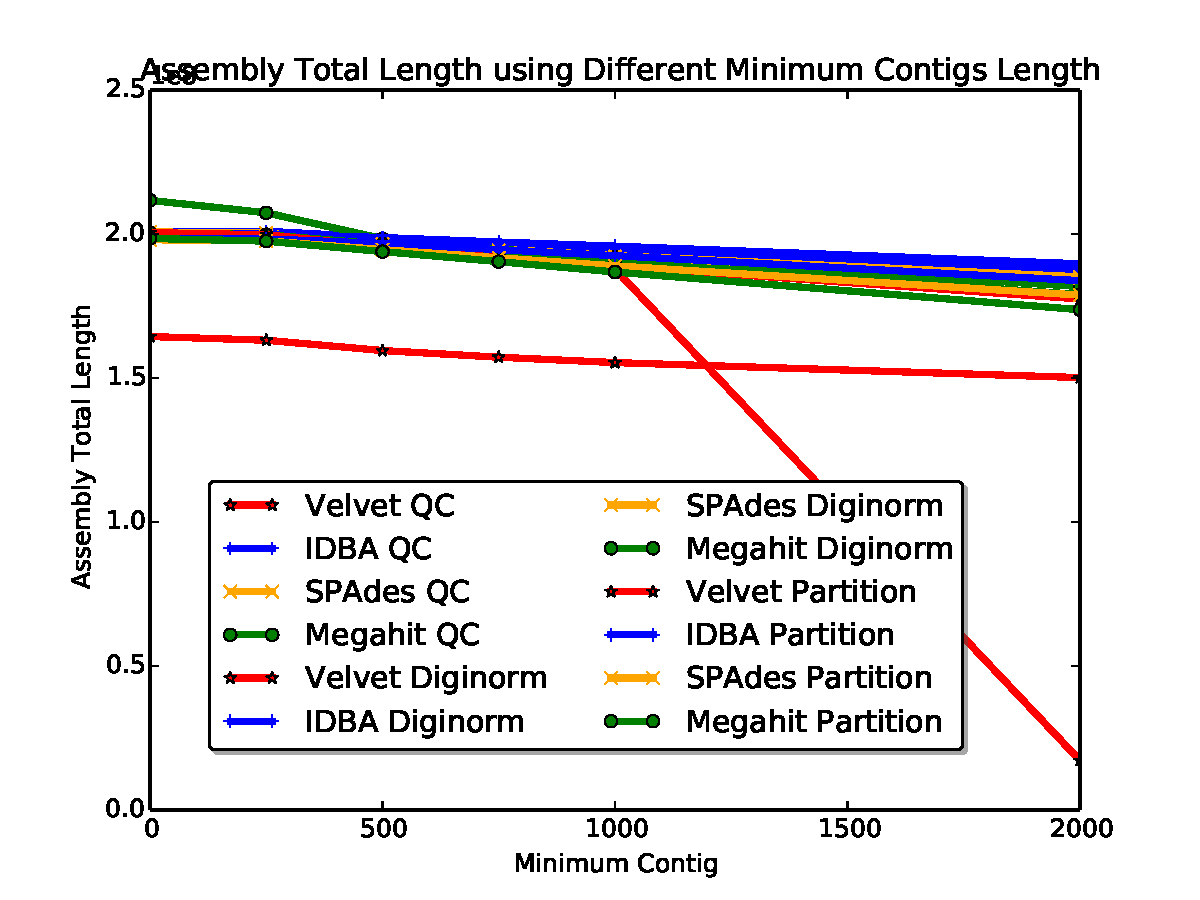
\includegraphics[height=3.2in,width=4.5in]{total-length-contigs.pdf}  
\caption{\small \sl Total Length of assemblies in basepairs based on different min contigs length.\label{fig:mincontig}}  
\end{center}  
\end{figure}  
 

\begin{figure} [h] 
\begin{center}  
 
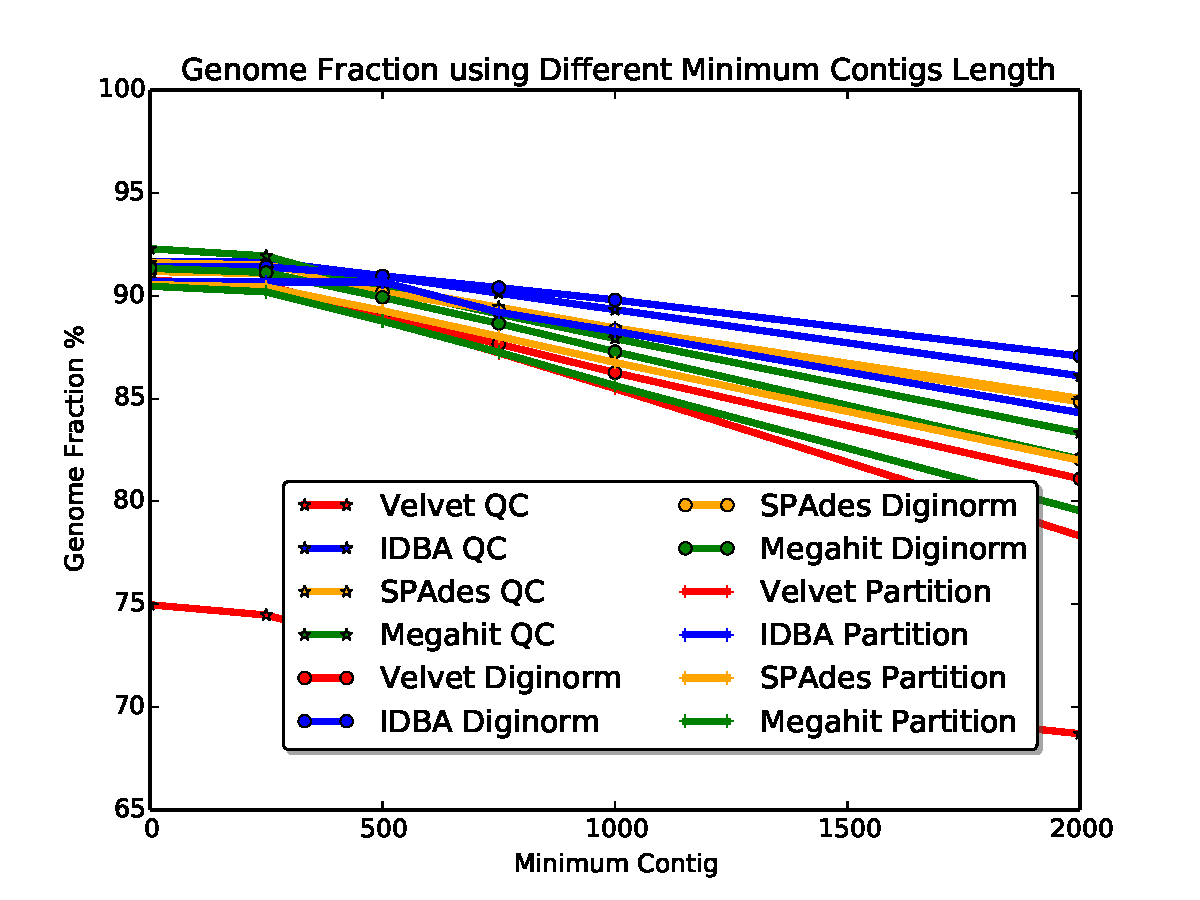
\includegraphics[height=3.2in,width=4.5in]{genome-fraction-contigs.pdf}  
\caption{\small \sl Genome Fraction of assemblies in basepairs based on different min contigs length.\label{fig:gf}}  
\end{center}  
\end{figure}  


\begin{figure} [h] 
\begin{center}  
 
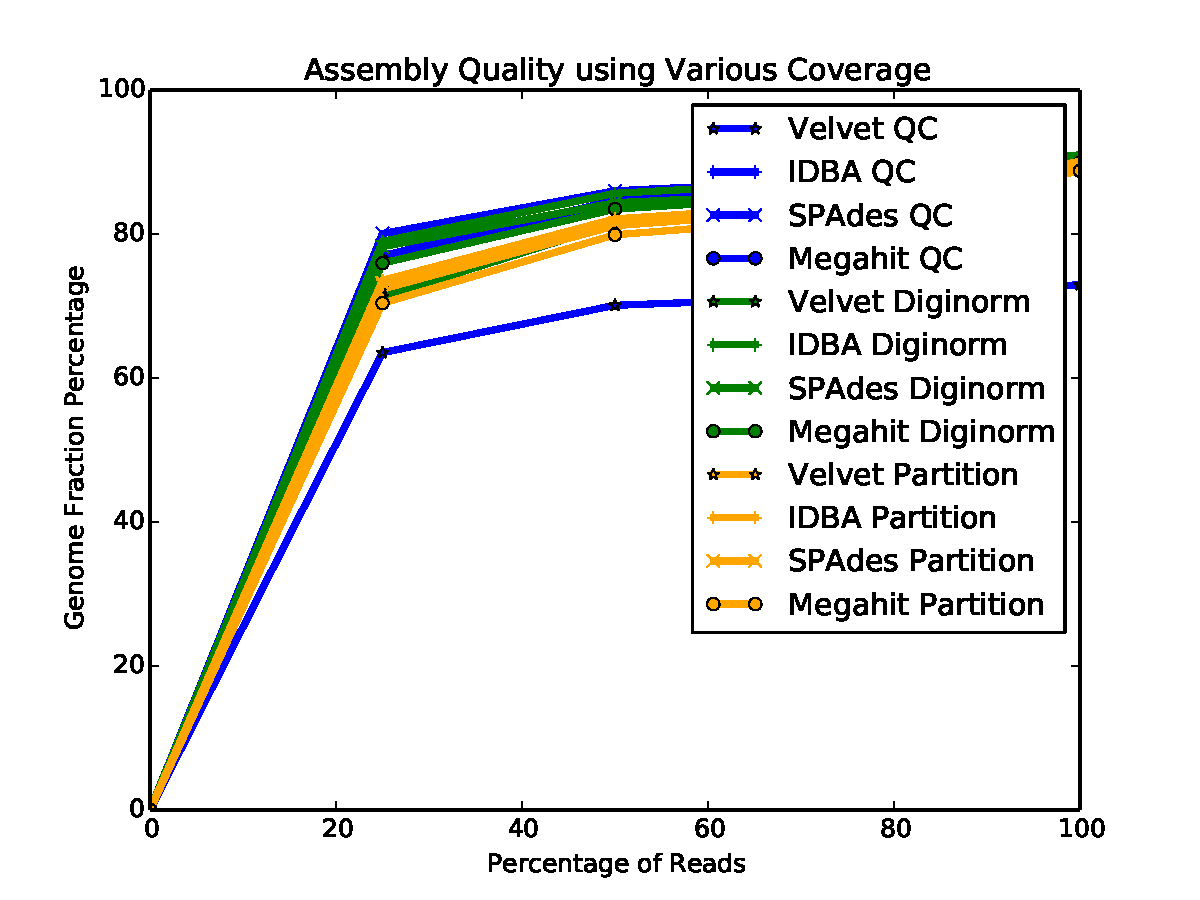
\includegraphics[height=3.2in,width=4.5in]{sampling.pdf}  
\caption{\small \sl Genome Fraction of assemblies using different read coverage.\label{fig:sampling}}  
\end{center}  
\end{figure}  
 

\begin{figure} [h] 
\begin{center}  
 
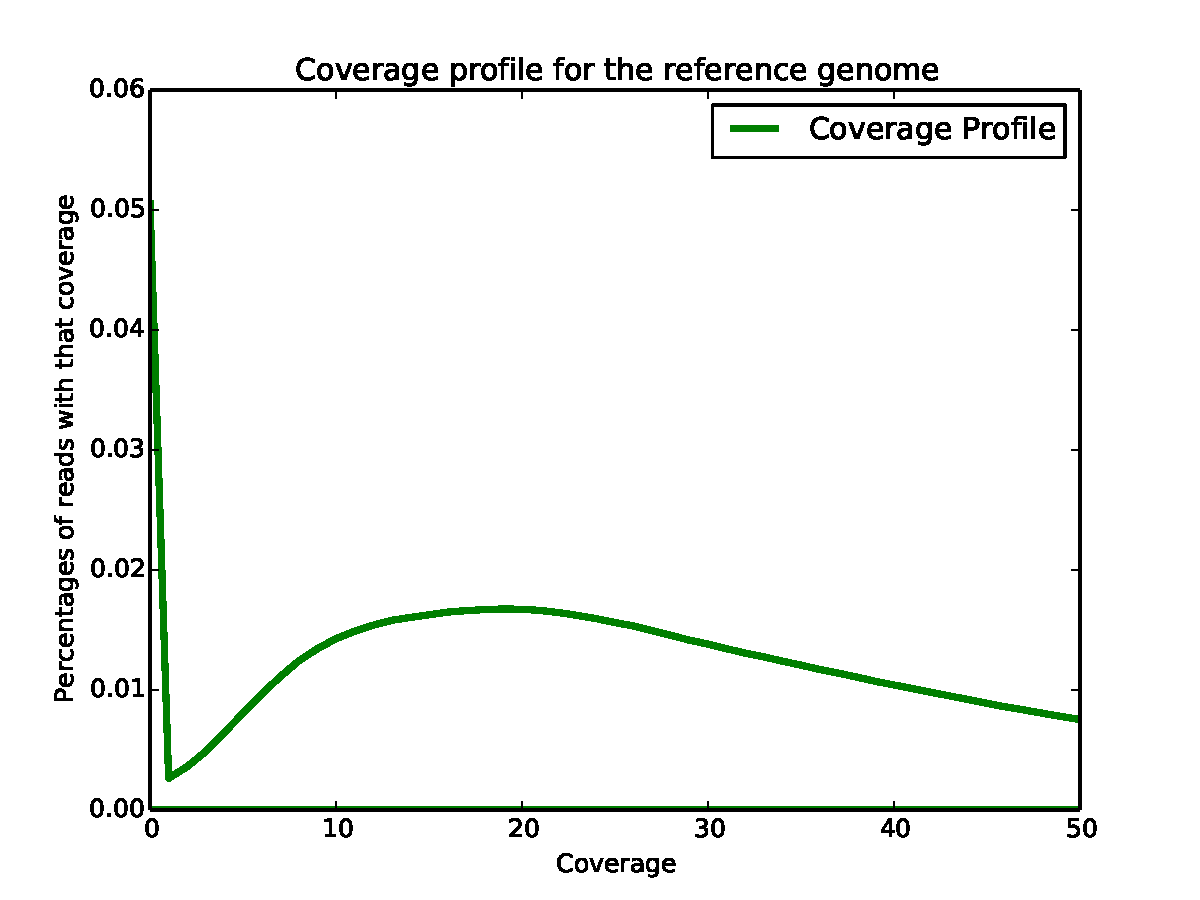
\includegraphics[height=3.2in,width=4.5in]{profilecoveragereads.pdf}  
\caption{\small \sl Reference genome coverage.\label{fig:coverage-profile}}  
\end{center}  
\end{figure} 


\begin{figure} [h] 
\begin{center}  
 
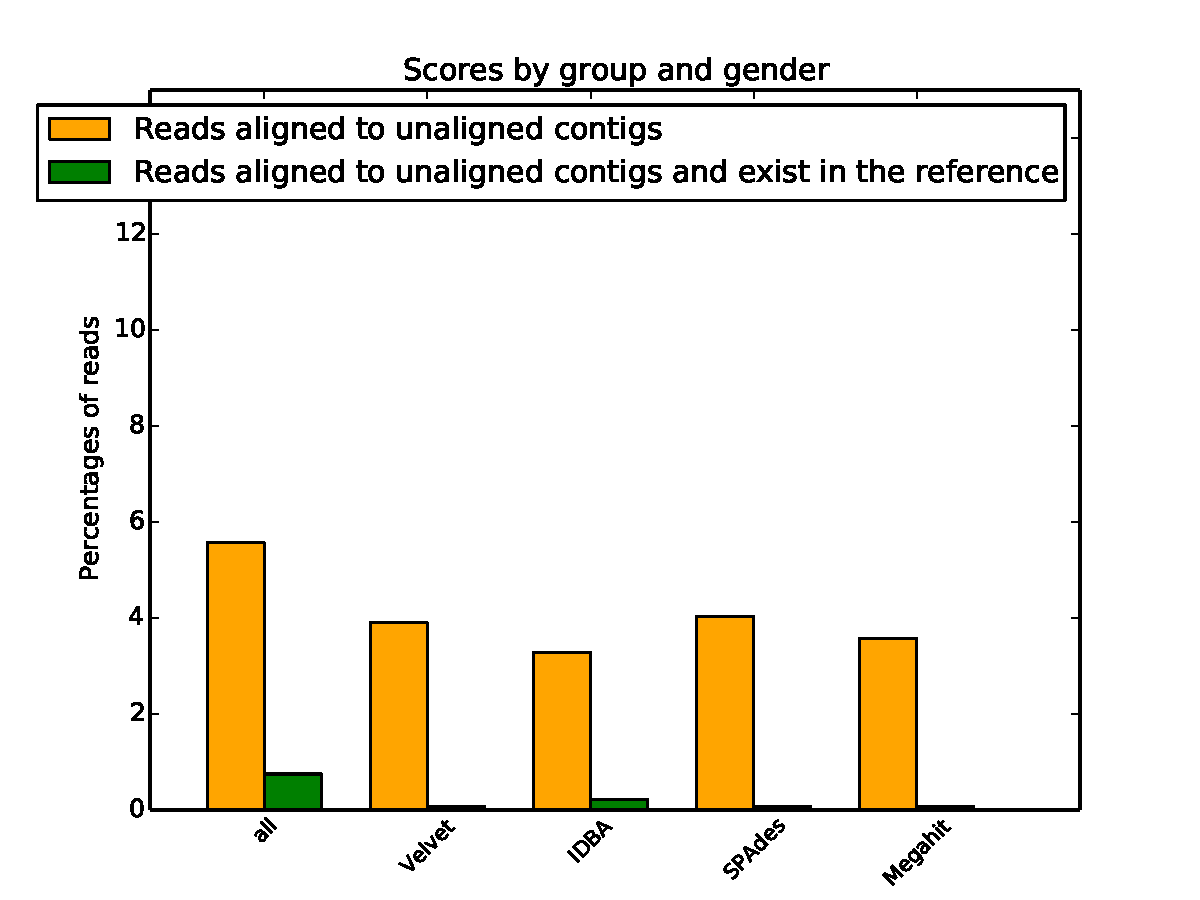
\includegraphics[height=3.2in,width=4.5in]{unaliged-hist.pdf}  
\caption{\small \sl Histogram for unaligned reads.\label{fig:unaliged-hist}}  
\end{center}  
\end{figure} 

\section*{Tables}
% 
% See introductory notes if you wish to include sideways tables.
%
% NOTE: Please look over our table guidelines at http://www.plosone.org/static/figureGuidelines#tables to make sure that your tables meet our requirements. Certain types of spacing, cell merging, and other formatting tricks may have unintended results and will be returned for revision.
%
%\begin{table}[!ht]
%\caption{
%\bf{Table title}}
%\begin{tabular}{|c|c|c|}
%table information
%\end{tabular}
%\begin{flushleft}Table caption
%\end{flushleft}
%\label{tab:label}
% \end{table}



%\begin{table}[t]
%\caption{Coverage Distribution}
%\centering
%\begin{tabular}{|c|c|}
%\hline
% \textbf{Coverage Range}& \textbf{No. of Reads}   \\ [0.5ex] % inserts table %heading
%\hline
%{ Between 20 and 40} & 95,540,661 \\
%\hline
%{ Between 40 and 60} &108,083 \\
%\hline
%{ Between 60 and 80} &22,677\\
%\hline
%{ Between 80 and 100} &17,148\\
%\hline
%{ Between 100 and 200} &80,878\\
%\hline
%{Coverage $\geq 200$} & 402,333\\
%\hline
%\end{tabular}
%\label{table:cov-dist} 
%\end{table}



\begin{table}[h]
\caption{Assembly Quality Metrics}
\centering
\begin{tabular}{|c|c|c|c|c|}
\hline
\textbf {Treatment/Quality Metric}& \textbf{Quality Filtering} & \textbf{Digital Normalization} & \textbf{Partition} \\ [0.5ex] % inserts table %heading
\hline
 \multicolumn{4}{|c|} {\textbf{(1) Velvet}}    \\ [0.5ex] % inserts table %heading
\hline
\textbf{Genome Fraction}& 72.949&89.043&88.879 \\
\hline
\textbf{Unaligned Length} &8,977,149&10,909,693&11,317,834\\ [1ex]
\hline
\textbf{Misassembled contigs length  }&16,566,891&25,594,315&16,922,852 \\ [1ex]
\hline
\textbf{N50} &38,028 &18,944 &8,504 \\ [1ex]
\hline
\textbf{NG50 }&22223&17212&7905  \\ [1ex]
\hline
\multicolumn{4}{|c|}{ \textbf{(2) IDBA-UD}}    \\ [0.5ex] % inserts table %heading
\hline
\textbf{Genome Fraction} &90.969&	91.003&90.082 \\   
\hline
\textbf{Unaligned Length}  &10,709,716&10,637,811&10,644,357 \\ [1ex]
\hline
\textbf{Misassembled contigs length  }&21,777,032&27,668,818&18,440,791  \\ [1ex]
\hline
\textbf{N50} &49773&47828&26575 \\ [1ex]
\hline
\textbf{NG50}&45748&44351&24326\\ [1ex]
\hline
\multicolumn{4}{|c|}{ \textbf{(3) SPAdes} }   \\ [0.5ex] % inserts table %heading
\hline
\textbf{Genome Fraction} &90.424&90.173&89.272\\
\hline
\textbf{Unaligned Length} &10,597,529&10,621,398&10,500,235 \\ [1ex]
\hline
\textbf{Misassembled contigs length  }&28,238,787&23,103,154&14,338,099  \\ [1ex]
\hline
\textbf{N50} &42773&35580&22319\\ [1ex]
\hline
\textbf{NG50} &38841&32598&19909\\ [1ex]
\hline
\multicolumn{4}{|c|}{ \textbf{(4) MEGAHIT} }    \\ [0.5ex] % inserts table %heading
\hline
\textbf{Genome Fraction} &90.358&89.92&88.769 \\
\hline
\textbf{Unaligned Length}&10,686,421&10,581,435&10,564,244 \\ [1ex]
\hline
\textbf{Misassembled contigs length  }&11,927,502&17,319,534&11,814,070 \\ [1ex]
\hline
\textbf{N50} &35,136&27,302&17,492 \\ [1ex]
\hline
\textbf{NG50} &32251&25248&15393 \\ [1ex]
\hline

\end{tabular}
\label{table:qualtiy-metrics}
\end{table}

\begin{table}[h]
\caption{Running Time and Memory Utilization}
\centering
\begin{tabular}{|c|c|c|c| }
\hline
\textbf {Treatment/Quality Metric}& \textbf{Quality Filtering} & \textbf{Digital Normalization} & \textbf{Partition}  \\ [0.5ex] % inserts table %heading
\hline
 \multicolumn{4}{|c|} {\textbf{(1) Velvet}}    \\ [0.5ex] % inserts table %heading
\hline
\textbf{Running Time} &60:42:52 &6:48:46 &4:30:36   \\ 
\hline
\textbf{Memory Utilization in GB}&98.40&52.67&35.23\\ 
\hline
\multicolumn{4}{|c|}{ \textbf{(2) IDBA-UD}}    \\ [0.5ex] % inserts table %heading
\hline
\textbf{Running Time} &33:53:46&6:34:24 &8:30:29  \\ 
\hline`
\textbf{Memory Utilization in GB}&123.84&99.88&89.25\\ 
\hline
\multicolumn{4}{|c|}{ \textbf{(3) SPADes} }   \\ [0.5ex] % inserts table %heading
\hline
\textbf{Running Time} &67:02:16&15:53:10&7:54:26  \\
\hline
\textbf{Memory Utilization in GB}&381.79&121.52&123.7 \\ 
\hline
\multicolumn{4}{|c|}{ \textbf{(4) MEGAHIT} }    \\ [0.5ex] % inserts table %heading
\hline
\textbf{Running Time}&1:52:55&0:30:23&1:23:28 \\
\hline
\textbf{Memory Utilization in GB}&33.41&18.89&189.55 \\ 
\hline


\end{tabular}
\label{table:time-memory}
\end{table}



\begin{table}[h]
\caption{mis-assemblies}
\centering
\begin{tabular}{|c|c|c|c|c|}
\hline
\textbf {Assembly}& \textbf{Quality Filtering} & \textbf{Digital Normalization} & \textbf{Partition} \\ [0.5ex] % inserts table %heading
\hline
 \multicolumn{4}{|c|} {\textbf{(1) Velvet}}    \\ [0.5ex] % inserts table %heading
\hline
\textbf{mis-assemblies}&917&5271&5202 \\
\hline
\textbf{Relocations} &592&998&1036 \\ [1ex]
\hline
\textbf{Translocations}&309&4262&4153  \\ [1ex]
\hline
\textbf{Inversions}&16&11&13  \\ [1ex]
\hline
\textbf{Misassembled Contigs Length}&16,566,891&25,594,315&16,922,852 \\ [1ex]
\hline
\textbf{Mismatches} &104,740&174,446&178,348  \\ [1ex]
\hline 
\textbf{Percentage of Mismatches}&0.05\%&0.08\%&0.09\%  \\[1ex]
\hline
\textbf{Indels Length}&50,190&181,453&346,988 \\ [1ex]
\hline
\textbf{Indels Percentage}&0.02\%&0.09\%&0.17\%\\ [1ex]
\hline

 \multicolumn{4}{|c|} {\textbf{(3) IDBA-UD}}    \\ [0.5ex] % inserts table %heading
\hline
\textbf{mis-assemblies}&1223&1094&960  \\
\hline
\textbf{Relocations} &613&668&578 \\ [1ex]
\hline
\textbf{Translocations}&580&398&350 \\ [1ex]
\hline
\textbf{Inversions} &30&28&32 \\ [1ex]
\hline
\textbf{Misassembled Contigs Length}&21,777,032&27,668,818&18,440,791 \\ [1ex]
\hline
\textbf{Mismatches} &162,733 &231,432&230,840 \\ [1ex]
\hline 
\textbf{Percentage of Mismatches}&0.08\%&0.11\%&0.11\% \\[1ex]
\hline
\textbf{Indels Length} &30,433&43,358&42,523  \\ [1ex]
\hline
\textbf{Indels Percentage}&0.01\%&0.02\%&0.02\%  \\ [1ex]
\hline


 \multicolumn{4}{|c|} {\textbf{(2) SPAdes}}    \\ [0.5ex] % inserts table %heading
\hline
\textbf{mis-assemblies}&894&997&753 \\
\hline
\textbf{Relocations}&608&613&496 \\ [1ex]
\hline
\textbf{Translocations}&267&368&239\\ [1ex]
\hline
\textbf{Inversions}&19&16&18\\ [1ex]
\hline
\textbf{Misassembled Contigs Length}&28,238,787&23,103,154&14,338,099\\ [1ex]
\hline
\textbf{Mismatches}&184,630&244,849&235,396\\ [1ex]
\hline 
\textbf{Percentage of Mismatches}&0.09\%&0.12\%&0.11\%\\ [1ex]
\hline
\textbf{Indels Length}&27,328&32,783&21,516\\ [1ex]
\hline
\textbf{Indels Percentage}&0.01\% &0.02\%&0.01\%\\ [1ex]
\hline

 \multicolumn{4}{|c|} {\textbf{(4) MEGAHIT}}    \\ [0.5ex] % inserts table %heading
\hline
\textbf{mis-assemblies}&738&880&748 \\
\hline
\textbf{Relocations}&448&593&513\\ [1ex]
\hline
\textbf{Translocations}&172&274&222\\ [1ex]
\hline
\textbf{Inversions}&118&13&13\\ [1ex]
\hline
\textbf{Misassembled Contigs Length}&11,927,502&17,319,534&11,814,070  \\ [1ex]
\hline
\textbf{Mismatches}&152,964&207,349&203,515\\ [1ex]
\hline 
\textbf{Percentage of Mismatches}&0.07\%&0.10\%&0.10\%\\[1 ex]
\hline
\textbf{Indels Length }&15,298&18,195&16,517\\ [1ex]
\hline
\textbf{Indels Percentage}&0.01\%&0.01\%&0.01\% \\ [1ex]
\hline
\end{tabular}
\label{table:mis-assemblies}
\end{table}

\begin{table}[t]
\caption{Mapping quality-filtered reads to assemblies}
\centering
\begin{tabular}{|c|c|c|c|}
\hline
\textbf {Treatment}& \textbf{Quality Filtering} & \textbf{Digital Normalization} & \textbf{Partition}  \\ [0.5ex] % inserts table %heading
\hline
 \multicolumn{4}{|c|} {\textbf{(1) Velvet}}    \\ [0.5ex] % inserts table %heading
\hline
\textbf{No. of Unaligned Sequences}&6,801,329&3,375,222&3,890,205  \\ 
\hline
\textbf{Percentage}&6.40\%&3.17\%&3.66\% \\
\hline
\multicolumn{4}{|c|}{ \textbf{(2) IDBA-UD}}    \\ [0.5ex] % inserts table %heading
\hline
\textbf{No. of Unaligned Sequences}&1,490,609&1,738,371&2,297,377 \\
\hline
\textbf{Percentage}&1.40\%&1.63\%&2.16\% \\
\hline
\multicolumn{4}{|c|}{ \textbf{(3) SPAdes} }   \\ [0.5ex] % inserts table %heading
\hline
\textbf{No. of Unaligned Sequences}&2,100,555&2,439,158&2,804,006\\
\hline
\textbf{Percentage}&1.98\%&2.29\%&2.64\%\\
\hline
\multicolumn{4}{|c|}{ \textbf{(4) MEGAHIT} }    \\ [0.5ex] % inserts table %heading
\hline
\textbf{No. of Unaligned Sequences}&1,559,300&2,082,881&2,747,427 \\
\hline
\textbf{Percentage}&1.47\%&1.96\% &2.58\% \\
\hline
\end{tabular}
\label{table:reads-mapping} 
\end{table}


\begin{table}[h]
\caption{Mapping unaligned  contigs to Idba quality-filtered  unaligned contigs }
\centering
\begin{tabular}{|c|c|c|c|c|}
\hline
\textbf {Treatment/Quality Metric}& \textbf{Quality Filtering} & \textbf{Digital Normalization} & \textbf{Partition} \\ [0.5ex] % inserts table %heading
\hline
 \multicolumn{4}{|c|} {\textbf{(1) Velvet}}    \\ [0.5ex] % inserts table %heading
\hline
\textbf{Unaligned IDBA Fraction}&80.613 \%&92.03\%&92.982\%   \\
\hline
\textbf{Unaligned Length}&2,475,529& 3192491&3,868,558 \\ [1ex]
\hline
\textbf{Percentage of unaligned}&37.06\%&47.8\%&57.92\%\\ [1ex]
\hline
\multicolumn{4}{|c|}{ \textbf{(2) IDBA-UD}}    \\ [0.5ex] % inserts table %heading
\hline
\textbf{Unaligned IDBA Fraction }&-&91.53\%&94.72\%\\   


\hline
\textbf{Unaligned Length}&-&498,299&1,320,036\\ [1ex]
\hline
\textbf{Percentage of unaligned}&-&7.46\%&19.76\% \\ [1ex]
\hline
\multicolumn{4}{|c|}{ \textbf{(3) SPAdes} }   \\ [0.5ex] % inserts table %heading
\hline
\textbf{Unaligned IDBA Fraction}&91.92\%&93.959\%&94.826\%\\
\hline
\textbf{Unaligned Length}&2,174,574&1,951,911&2,398,664\\ [1ex]
\hline
\textbf{Percentage of unaligned}&32.56\%&29.22\%&35.91\%\\ [1ex]
\hline
\multicolumn{4}{|c|}{ \textbf{(4) MEGAHIT} }    \\ [0.5ex] % inserts table %heading
\hline
\textbf{Unaligned IDBA Fraction}&92.715\%&91.838\%&92.219\% \\
\hline
\textbf{Unaligned Length}&916,247&1,569,436&3,832,050 \\ [1ex]
\hline
\textbf{Percentage of unaligned}&13.72\%&23.5\%&57.37\%\\ [1ex]
\hline
\end{tabular}
\label{table:unaligned-mapping}
\end{table}


%%%%%SUPLEMENTARY TABLES 
\begin{table}[h]
\caption{Supplementary Table: More Assembly Quality Metrics}
\centering
\begin{tabular}{|c|c|c|c|c|}
\hline
\textbf {Treatment/Quality Metric}& \textbf{Quality Filtering} & \textbf{Digital Normalization} & \textbf{Partition} \\ [0.5ex] % inserts table %heading
\hline
 \multicolumn{4}{|c|} {\textbf{(1) Velvet}}    \\ [0.5ex] % inserts table %heading
\hline
\textbf{N75}&13301&6084&3771\\ [1ex]
\hline
\textbf{NG75}&1186&4805&3214\\ [1ex]
\hline
\textbf{L50} &1013&2455&6037 \\ [1ex]
\hline
\textbf{LG50} &1806&2740&6641\\ [1ex]
\hline
\textbf{L75} &2777&7026&14734\\ [1ex]
\hline
\textbf{LG75} &11087&8460&16867\\ [1ex]
\hline
\multicolumn{4}{|c|}{ \textbf{(2) IDBA-UD}}    \\ [0.5ex] % inserts table %heading
\hline
\textbf{N75}&11693&12154&7834  \\ [1ex]
\hline
\textbf{NG75} &9617	&10221&6461 \\ [1ex]
\hline
\textbf{L50}&828&896&1536\\ [1ex]
\hline
\textbf{LG50}&899&970&1712 \\ [1ex]
\hline
\textbf{L75}&2986&3025&5062 \\ [1ex]
\hline
\textbf{LG75}&3467&3484	&6002\\ [1ex]
\hline
\multicolumn{4}{|c|}{ \textbf{(2) SPAdes}}    \\ [0.5ex] % inserts table %heading
\hline
\textbf{N75} &11263&10554&6900\\ [1ex]
\hline
\textbf{NG75} &9005	&8379&5401\\ [1ex]
\hline
\textbf{L50} &974&1192&1846\\ [1ex]
\hline
\textbf{LG50} &1078&1325&2108\\ [1ex]
\hline
\textbf{L75} &3276&3768&5840\\ [1ex]
\hline
\textbf{LG75} &3908&4495&7198\\ [1ex]
\hline
\multicolumn{4}{|c|}{ \textbf{(4) MEGAHIT} }    \\ [0.5ex] % inserts table %heading
\hline
\textbf{N75} &8166&7230&5271 \\ [1ex]
\hline
\textbf{NG75} &6601	&5632&4030 \\ [1ex]
\hline
\textbf{L50} &1199	&1582&2490 \\ [1ex]
\hline
\textbf{LG50} &1306	&1757&2848 \\ [1ex]
\hline
\textbf{L75} &4164	&5063&7670 \\ [1ex]
\hline
\textbf{LG75} &4907&6147&9581 \\ [1ex]
\hline

\end{tabular}
\label{table:sub-qc}
\end{table}


\begin{table}[t]
\caption{Comparision between N50 and NG50}
\centering
\begin{tabular}{|c|c|c|c|}
\hline
\textbf {Treatment}& \textbf{Quality Filtering} & \textbf{Digital Normalization} & \textbf{Partition}  \\ [0.5ex] % inserts table %heading
\hline

 \multicolumn{4}{|c|} {\textbf{(1) Velvet}}    \\ [0.5ex] % inserts table %heading
\hline
\textbf{N50}&38,028&18,944&8,504 \\ 
\hline
\textbf{NG50}&22,223&17,212&7,905\\
\hline
 \multicolumn{4}{|c|} {\textbf{(2) IDBA-UD}}    \\ [0.5ex] % inserts table %heading
\hline
\textbf{N50}&49,773&47,828&26,575 \\ 
\hline
\textbf{NG50}&45,748&44,351&24,326 \\
\hline
 \multicolumn{4}{|c|} {\textbf{(3) SPAdes}}    \\ [0.5ex] % inserts table %heading
\hline
\textbf{N50}&42,773&35,580&22,319\\ 
\hline
\textbf{NG50}&38,841&32,598&19,909\\
\hline
 \multicolumn{4}{|c|} {\textbf{(4) MEGAHIT}}    \\ [0.5ex] % inserts table %heading
\hline
\textbf{N50}&35,136&27,302&17,492\\ 
\hline
\textbf{NG50}&32,251&25,248&15,393\\
\hline
\end{tabular}
\label{table:n50-ng50} 
\end{table}




 \section *{Supporting Information Legends} 
%
% Please enter your Supporting Information captions below in the following format:
%\item{\bf Figure SX. Enter mandatory title here.} Enter optional descriptive information here.
% 
%\begin{description}
%\item {\bf}
%\item {\bf}
%\end{description}

\end{document}

